\sectino*{Anhang}

\subsubsection{Aufgabenstellung original}

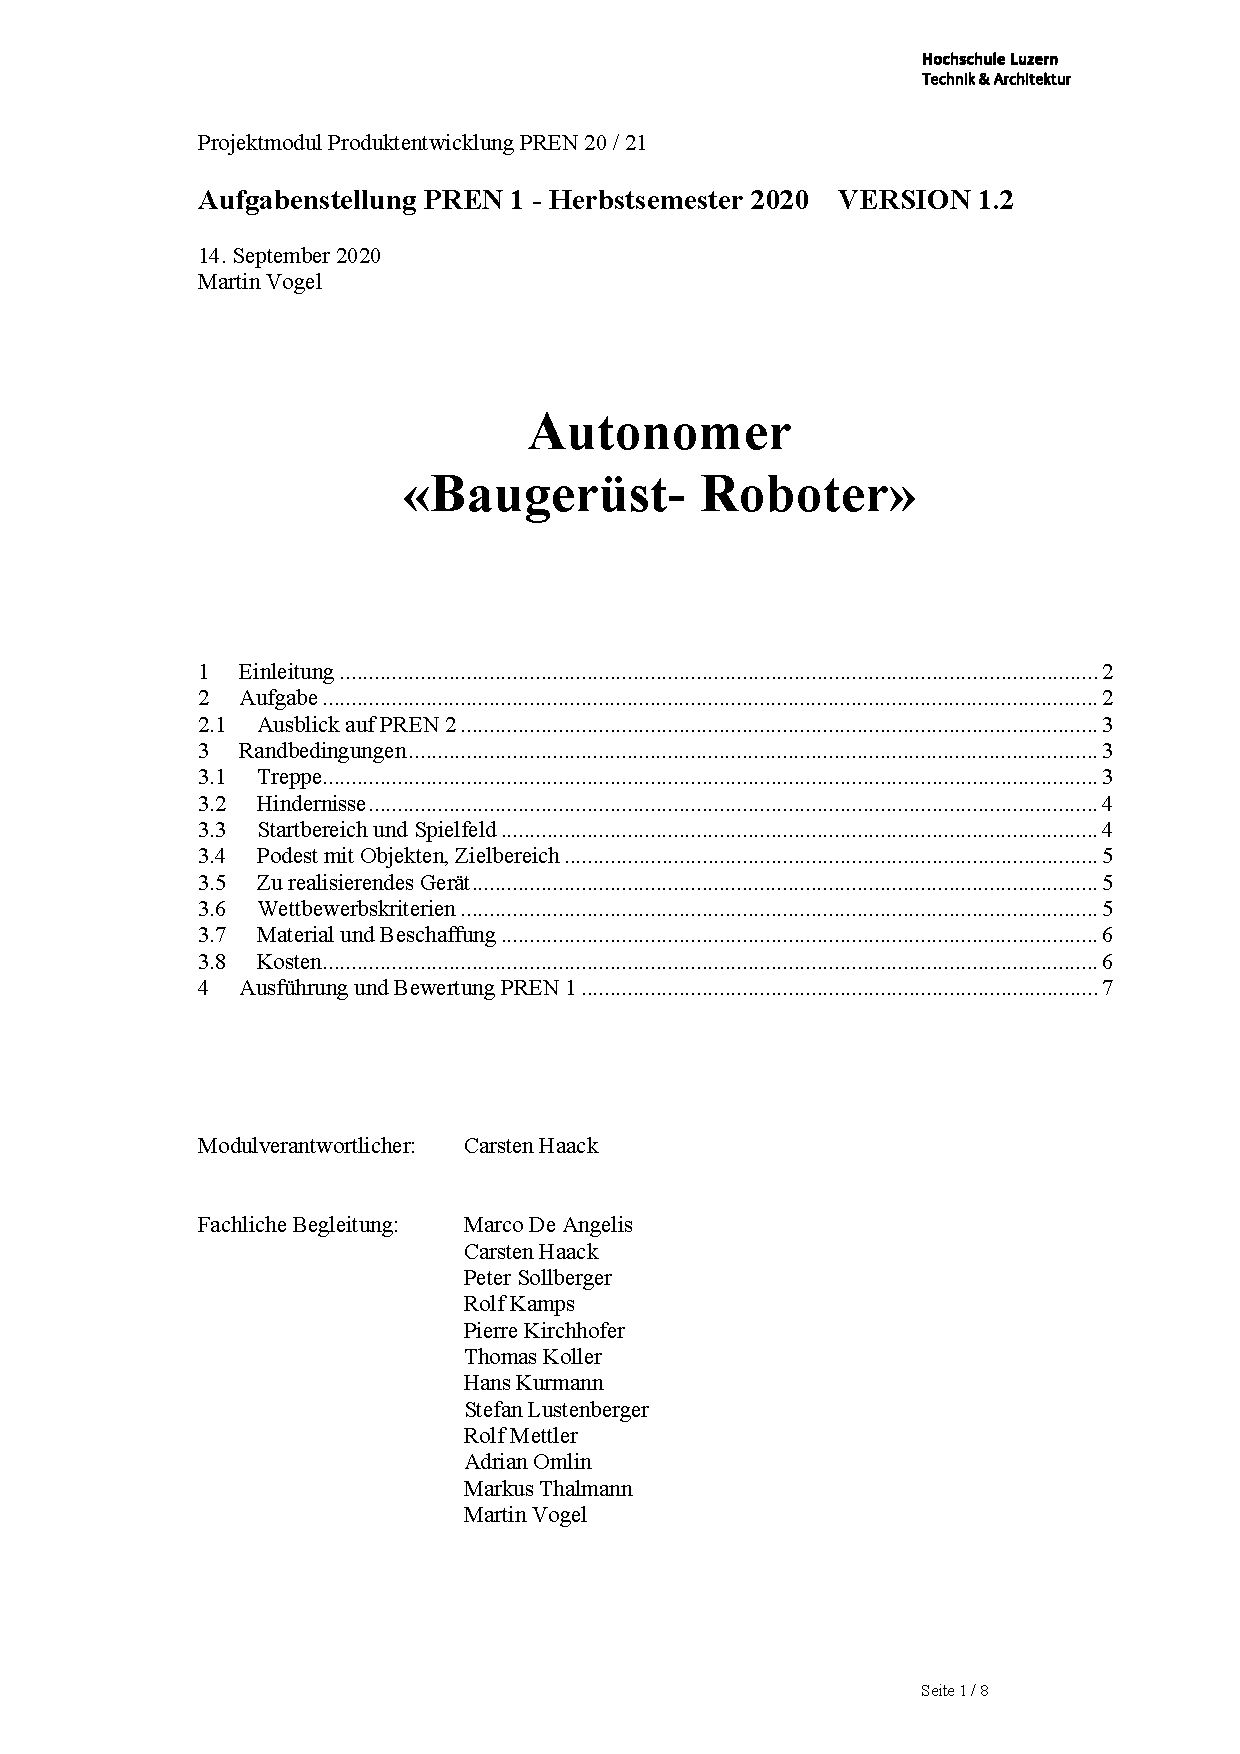
\includepdf[
  pages={1-},
  scale=1,
  pagecommand={\pagestyle{fancy}}
]{assets/Aufgabenstellung_PREN1_H20_v1_2.pdf}

\subsubsection{Berechnungen}

\textbf{Abmasse}

Anhand der vorgegebenen Treppe werden erste Massabschätzungen gemacht. Dabei werden die Tritthöhe und die Tritttiefe berücksichtigt.

\begin{figure}[H]
  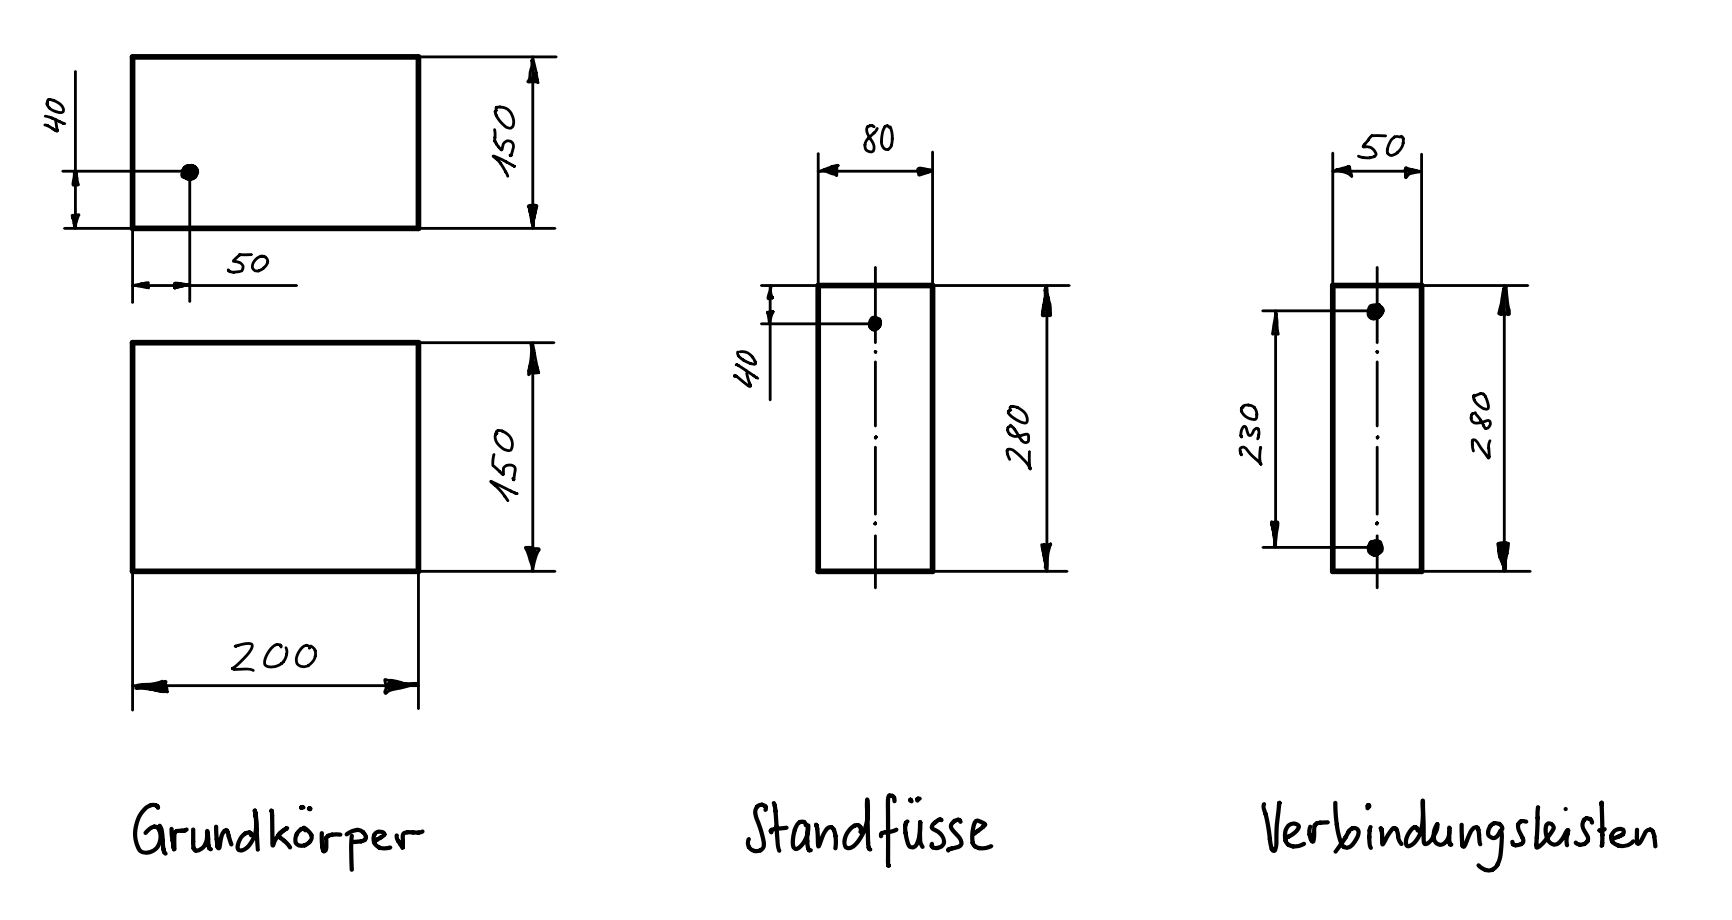
\includegraphics[width=1
  \textwidth]{img/Treppensteigen/Erste Abmasse}
  \centering
  \caption{Skizze erste Abmasse}
\end{figure}

\textbf{Berechnung der Massen und ihre Schwerpunkte}\\

\textbf{Grundkörper}

Für die Masse und den Schwerpunkt des Grundkörpers wurde eine Berechnung mit den Hauptkomponenten gemacht. Dabei wurden Halterungen, Sensoren, Kameras und Normteile wie Schrauben oder Passfedern nicht berücksichtigt.

Masse Grundplatte: 0.15 kg
Masse Welle 1: 0.6 kg
Masse Welle 3: 0.3 kg
Masse Motor 1: 0.3 kg
Masse Motor 2: 0.3 kg
Masse Akku: 0.074 kg
Zusatzmasse: 0.95 kg

Gesamt Masse Grundkörper: 2.9 kg

Schwerpunkt Grundplatte: 100 mm
Schwerpunkt Welle 1: 50 mm
Schwerpunkt Welle 3: 79.4 mm
Schwerpunkt Motor 1(ink. Halterung und Abtriebszahnrad): 79.4 mm
Schwerpunkt Motor 2(ink. Halterung und Abtriebszahnrad): 18 mm
Schwerpunkt Akku: 180 mm
Schwerpunkt Zusatzmasse: 180 mm

Schwerpunkt Grundkörper: 105.2 mm

Bild CAD

\textbf{Standfüsse}

Masse Standfuss: 0.51 kg
Schwerpunkt Standfuss: 184.8 mm

Bild CAD

\textbf{Verbindungsleisten}

Der Schwerpunkt der Verbindungsleisten wurde mittig gesetzt, um die Schwerpunktsberechnung zu vereinfachen.

Masse Verbindungsleisten: 0.18 kg
Schwerpunkt Verbindungsleisten: 140 mm

Bild CAD

\textbf{Notwendige Momente bei den Hubbewegungen}

Die Momente, die gebraucht werden, konnten mit den ersten Abmassen, Massen und Schwerpunkten der komponenten berechnet werden und dienen als Grundlage zur Auswahl der Motoren.

\textbf{Momente bei den Hubbewegungen:}

\textbf{1. Hubbewegung:}

Drehachse 1: Moment zum horizontalen Halten des Grundkörpers
\begin{align*}
    M_{Achse 1} &= F_{GG} * 0.0552\ m \\
    &= m_{GG} * g * 0.0552\ m \\
    &= 2.9\ kg * 9.81\ m/s^2\ * 0.0552\ m \\
    &= \underline{\underline{1.6\ Nm}}
\end{align*}

Drehachse 2: grösstes Moment am Anfang, in Ausgangsstellung
\begin{align*}
    M_{Achse 2} &= F_{GL} * 0.115\ m + F_{GG} * 0.1748\ m \\
    &= g * (m_{GL} * 0.115\ m + m_{GG} * 0.1748\ m \\
    &= 9.81\ m/s^2\ * (0.38\ kg * 0.115\ m + 2.9\ kg * 0.1748\ m) \\
    &= \underline{\underline{5.4\ Nm}}
\end{align*}

\textbf{2. Hubbewegung:}

Drehachse 1: grösstes Moment, wenn alle Teile horizontal
\begin{align*}
    M_{Achse 1} &= F_{GS} * 0.2852\ m + F_{GL} * 0.115\ m \\
    &= g * (m_{GS} * 0.2852\ m + m_{GL} * 0.115\ m) \\
    &= 9.81\ m/s^2 * (1.2\ kg * 0.2852\ m + 0.38\ kg * 0.115\ m) \\
    &= \underline{\underline{3.8\ Nm}}
\end{align*}

Drehachse 2: grösstes Moment, wenn Standfüsse horizontal
\begin{align*}
    M_{Achse 2} &= F_{GS} * 0.0552\ m \\
    &= m_{GS} * g * 0.0552\ m \\
    &= 1.02\ kg * 9.81\ m/s^2 * 0.0552\ m \\
    &=\underline{\underline{0.6\ Nm}}
\end{align*}

Motor 1 liefert das Moment, dass in der 1. Drehachse wirkt und Motor 2 liefert das Moment, dass in der 2. Drehachse wirkt.\\
\\
M$_{erforderlich}$ Achse 1: 5 Nm\\

M$_{erforderlich}$ Achse 2: 2.4 Nm





\subsection*{Detailrecherche}

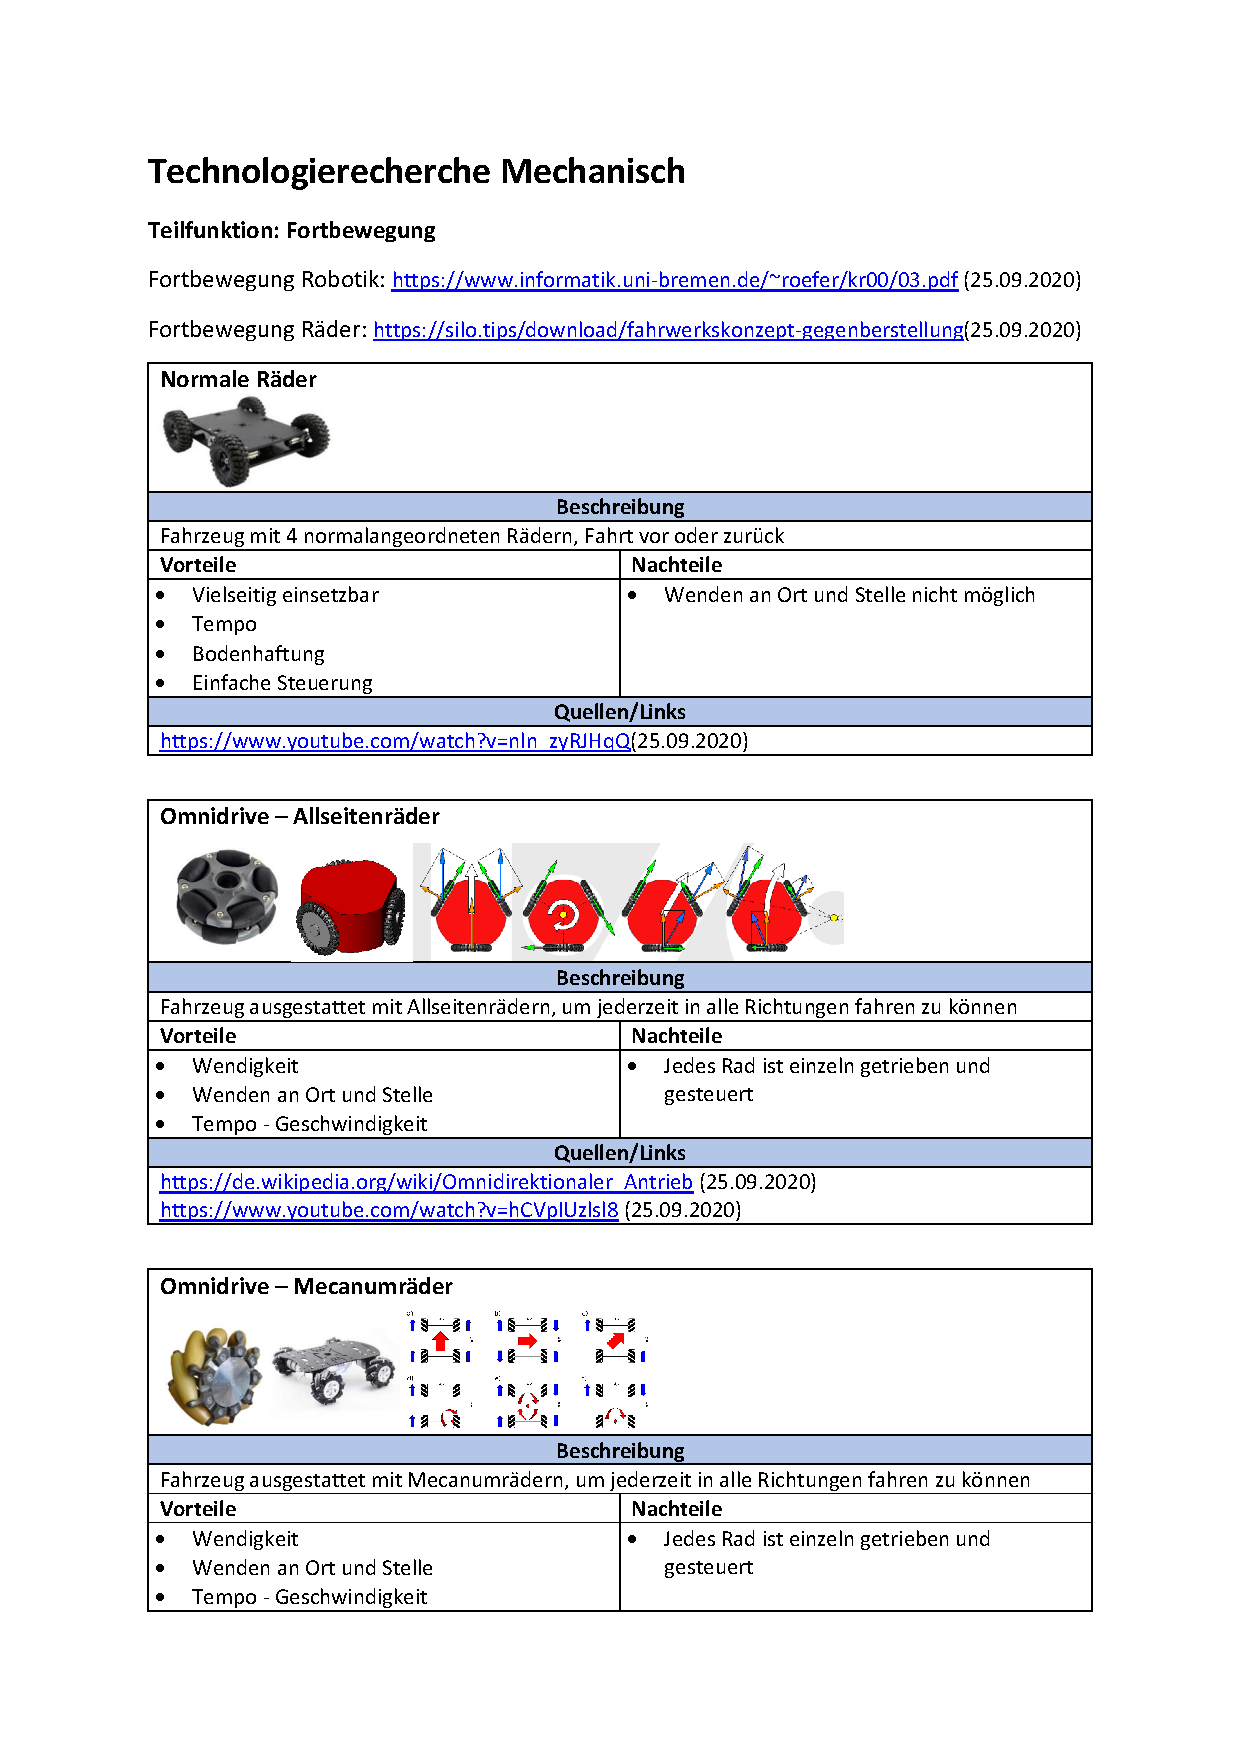
\includepdf[
  pages={1-},
  scale=1,
  pagecommand={\pagestyle{fancy}}
]{assets/Technologierecherche M.pdf}

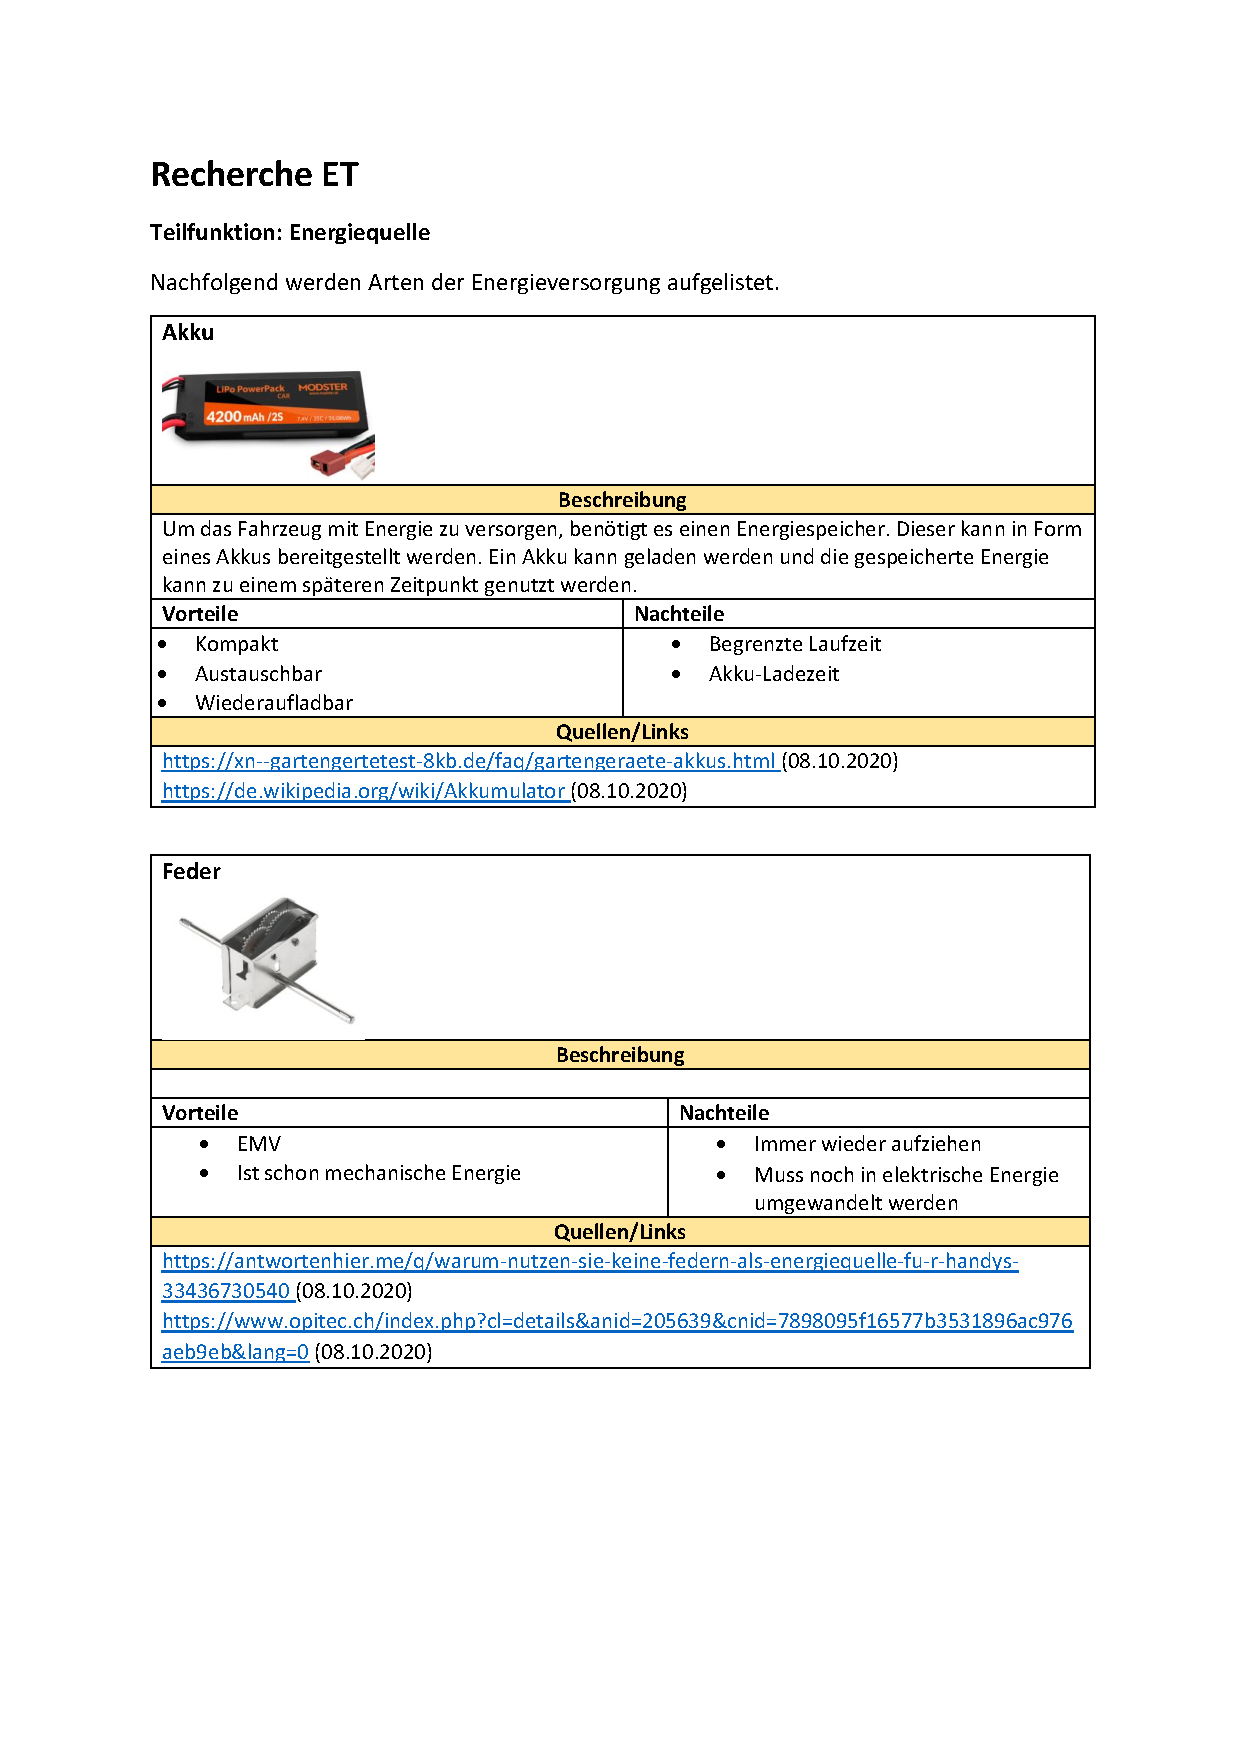
\includepdf[
  pages={1-},
  scale=1,
  pagecommand={\pagestyle{fancy}}
]{assets/Technologierecherche ET.pdf}

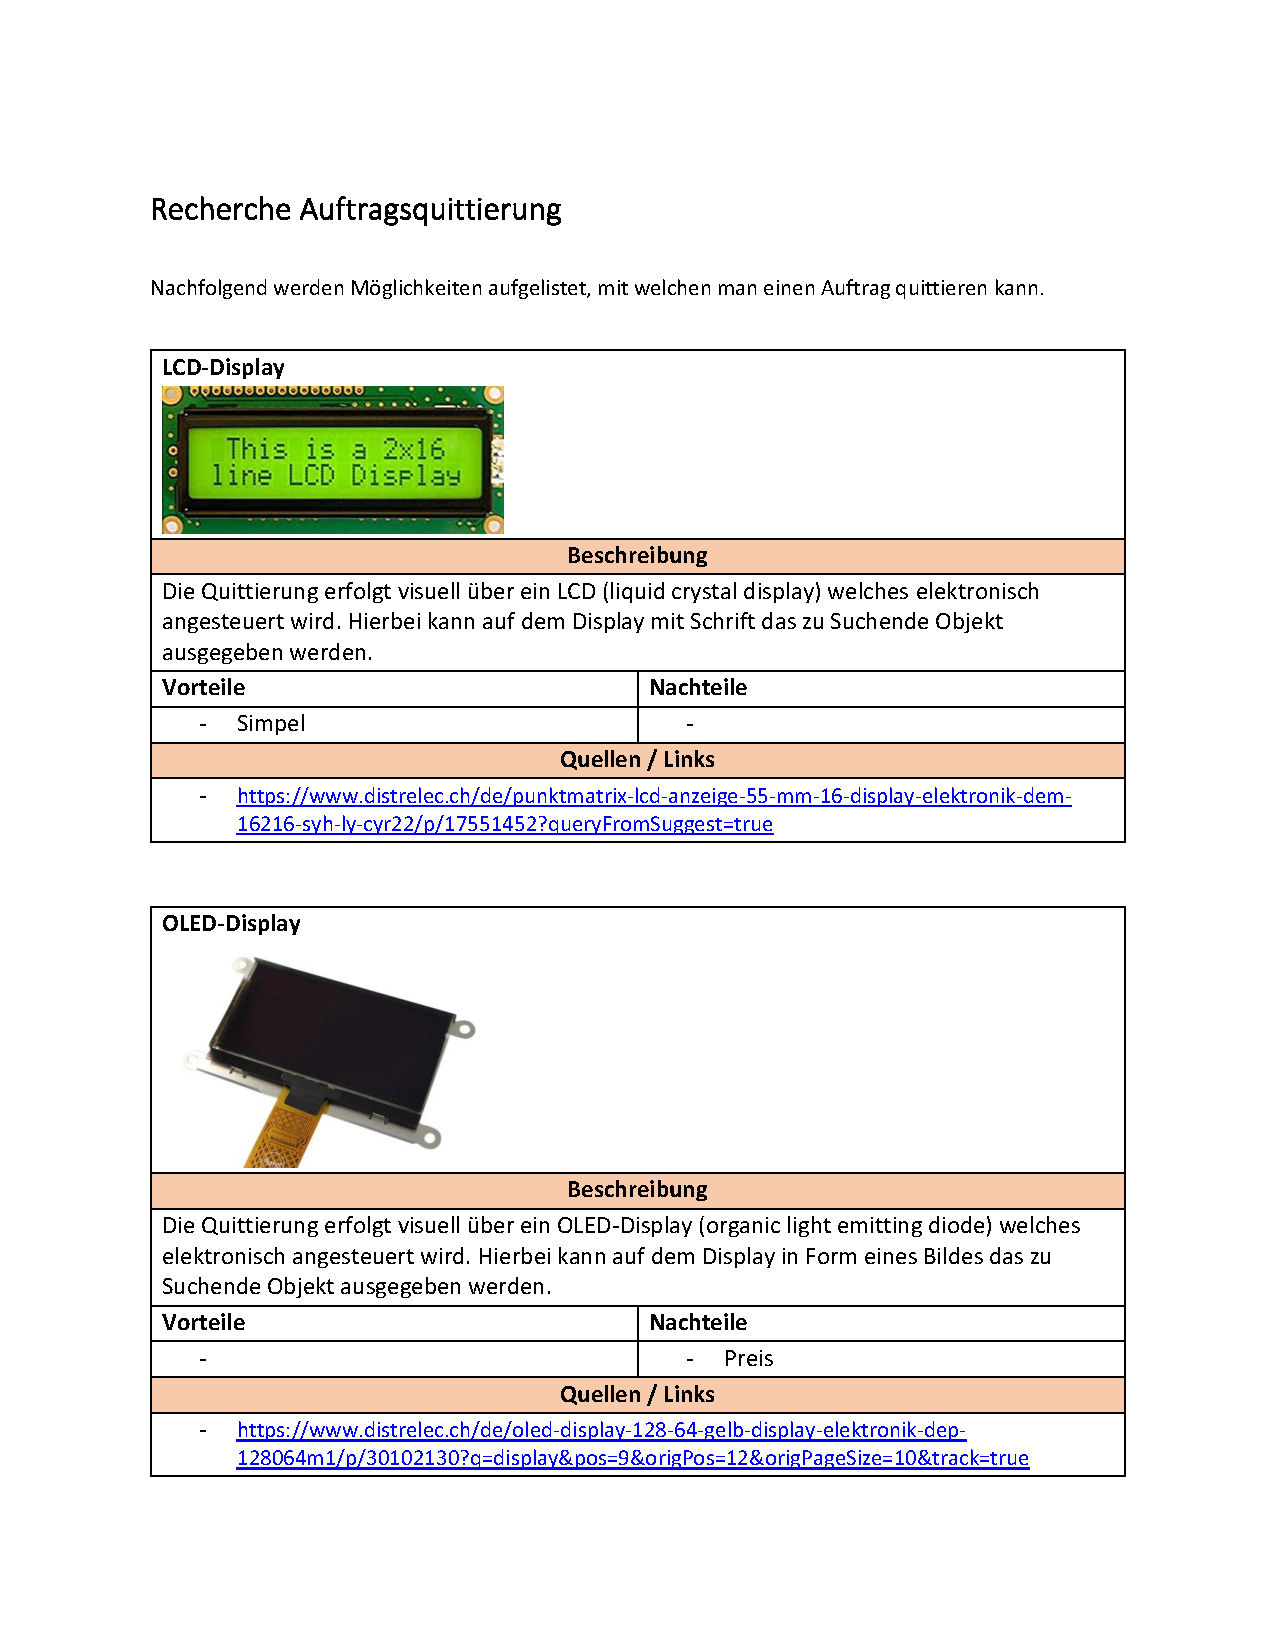
\includepdf[
  pages={1-},
  scale=1,
  pagecommand={\pagestyle{fancy}}
]{assets/Recherche Auftragsquittierung.pdf}


\includepdf[
  pages={1-},
  scale=1,
  pagecommand={\pagestyle{fancy}}
]{assets/Recherche Umgebungserkennung.pdf}